\documentclass[tikz,border=10pt]{standalone}
\usepackage{tikz}
\usepackage{fontawesome5}
\usepackage{amsmath,amssymb}
\usetikzlibrary{arrows.meta,positioning,fit,backgrounds,calc,shadows,shapes.geometric}

\definecolor{civNavy}{RGB}{15, 34, 64}
\definecolor{civBlue}{RGB}{28, 80, 160}
\definecolor{civTeal}{RGB}{14, 130, 120}
\definecolor{civLightBlue}{RGB}{238, 245, 255}
\definecolor{civBorder}{RGB}{185, 210, 240}
\definecolor{civGold}{RGB}{217, 119, 6}
\definecolor{civGreen}{RGB}{22, 130, 80}
\definecolor{civDark}{RGB}{20, 28, 42}
\definecolor{cInput}{RGB}{240, 246, 255}
\definecolor{cStem}{RGB}{224, 242, 254}
\definecolor{cStage1}{RGB}{209, 250, 229}
\definecolor{cStage2}{RGB}{254, 243, 199}
\definecolor{cStage3}{RGB}{254, 226, 226}
\definecolor{cStage4}{RGB}{236, 254, 255}

\begin{document}
% System Operational Flowchart for CiviQ
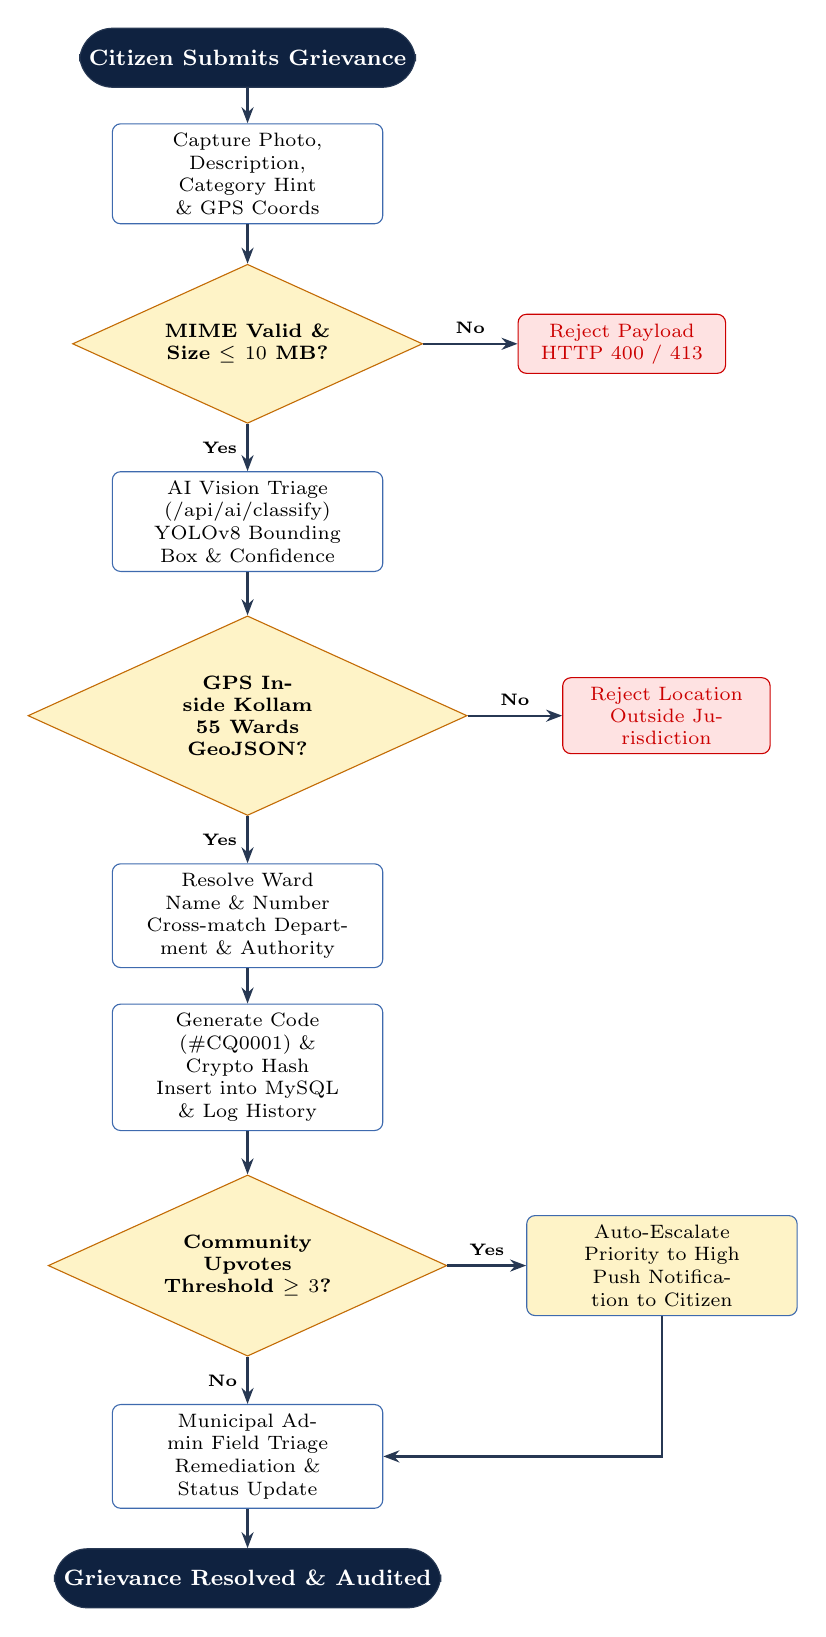
\begin{tikzpicture}[
    x=1cm, y=1cm,
    font=\sffamily,
    startstop/.style={
        rectangle, rounded corners=12pt, minimum width=2.8cm, minimum height=0.75cm,
        text centered, draw=civNavy!90, fill=civNavy, text=white,
        font=\fontsize{7.8}{9.2}\selectfont\bfseries
    },
    process/.style={
        rectangle, rounded corners=3pt, minimum width=3.4cm, minimum height=0.85cm,
        text centered, text width=3.2cm, draw=civBlue!85, fill=white,
        font=\fontsize{7.0}{8.2}\selectfont
    },
    decision/.style={
        diamond, aspect=2.2, minimum width=3.0cm, minimum height=0.9cm,
        text centered, text width=2.6cm, draw=civGold!90!black, fill=cStage2,
        font=\fontsize{6.8}{8.0}\selectfont\bfseries
    },
    errorbox/.style={
        rectangle, rounded corners=3pt, minimum width=2.6cm, minimum height=0.75cm,
        text centered, text width=2.4cm, draw=red!80!black, fill=cStage3,
        font=\fontsize{6.8}{8.0}\selectfont\color{red!80!black}
    },
    flowarr/.style={
        -{Stealth[scale=0.85]}, line width=0.85pt, draw=civNavy!90
    }
]

    % Nodes Placement
    \node (start) [startstop] at (0, 10.2) {Citizen Submits Grievance};
    \node (pingest) [process, below=0.45cm of start] {Capture Photo, Description,\\Category Hint \& GPS Coords};
    
    \node (dmime) [decision, below=0.5cm of pingest] {MIME Valid \&\\Size $\le 10$ MB?};
    \node (errmime) [errorbox, right=1.2cm of dmime] {Reject Payload\\HTTP 400 / 413};

    \node (pai) [process, below=0.6cm of dmime] {AI Vision Triage (/api/ai/classify)\\YOLOv8 Bounding Box \& Confidence};

    \node (dward) [decision, below=0.55cm of pai] {GPS Inside Kollam\\55 Wards GeoJSON?};
    \node (errward) [errorbox, right=1.2cm of dward] {Reject Location\\Outside Jurisdiction};

    \node (proute) [process, below=0.6cm of dward] {Resolve Ward Name \& Number\\Cross-match Department \& Authority};

    \node (pcommit) [process, below=0.45cm of proute] {Generate Code (\#CQ0001) \& Crypto Hash\\Insert into MySQL \& Log History};

    \node (dupvote) [decision, below=0.55cm of pcommit] {Community Upvotes\\Threshold $\ge 3$?};
    \node (pescl) [process, right=1.0cm of dupvote, fill=cStage2] {Auto-Escalate Priority to High\\Push Notification to Citizen};

    \node (padmin) [process, below=0.6cm of dupvote] {Municipal Admin Field Triage\\Remediation \& Status Update};

    \node (stop) [startstop, below=0.5cm of padmin] {Grievance Resolved \& Audited};

    % Arrows
    \draw [flowarr] (start) -- (pingest);
    \draw [flowarr] (pingest) -- (dmime);
    \draw [flowarr] (dmime) -- node[left, font=\fontsize{6.5}{7.5}\selectfont\bfseries] {Yes} (pai);
    \draw [flowarr] (dmime) -- node[above, font=\fontsize{6.5}{7.5}\selectfont\bfseries] {No} (errmime);
    
    \draw [flowarr] (pai) -- (dward);
    \draw [flowarr] (dward) -- node[left, font=\fontsize{6.5}{7.5}\selectfont\bfseries] {Yes} (proute);
    \draw [flowarr] (dward) -- node[above, font=\fontsize{6.5}{7.5}\selectfont\bfseries] {No} (errward);

    \draw [flowarr] (proute) -- (pcommit);
    \draw [flowarr] (pcommit) -- (dupvote);

    \draw [flowarr] (dupvote) -- node[above, font=\fontsize{6.5}{7.5}\selectfont\bfseries] {Yes} (pescl);
    \draw [flowarr] (dupvote) -- node[left, font=\fontsize{6.5}{7.5}\selectfont\bfseries] {No} (padmin);
    \draw [flowarr] (pescl) |- (padmin);

    \draw [flowarr] (padmin) -- (stop);

\end{tikzpicture}
\end{document}
